%\let\textcircled=\pgftextcircled
\chapter{Input data cleaning}
\label{chap:input_data_cleaning}

Input data from sensors doesn't represent real measure of vehicle physics quantities. Instruments have an error of measure, each one with different possible causes. This chapter deals with techniques used in the project to reduce that error, whether is caused by human accidentally or it's intrinsic of the sensor.

\section{Stationary time detection}
Most of the solutions to remove errors explained later are based on assumption on vehicle state. One of the most used assumption is when vehicle is stationary. \\
This can't be detected by a near zero acceleration along all axis because vehicle could be moving with constant speed. So integrated speed should be used, but integrating acceleration vectors that need corrections can bring next code logic to make mistakes as well being a waste of time because integration should be remade after having applied corrections. \\
One solution can be using non-directional speed from input data, calculated from GNSS data by the measure device in the box. But this speed is under effect of Kalman filters that react late to changes, still for trying to avoid measurement errors. One can derivate numerically the GNSS position to get a more precise speed and on top of that calculate stationary times. The choice of using speed subject to kalman filters or the one derived should be based on gnss sensor precision. Expecially when vehicle is stopped gnss error can be relevant as showed in the following picture.
\begin{figure}[H]
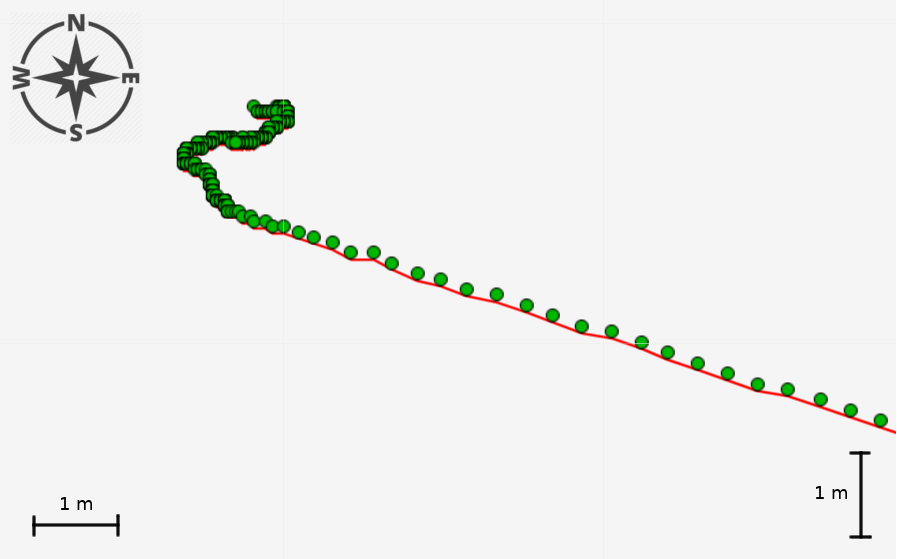
\includegraphics[width=\textwidth]{gnss_error_stationary_vehicle}
\caption{Green points represent gnss positions. On top-left gnss error can be noticed on a situation where vehicle was stationary in reality}
\end{figure}
To try to handle input data where vehicle never really stop, the algorithm for stationary time detection searches with and increasing threshold until enough moments are found.

\section{Gyroscope drift}
Gyroscopes have a drift that is unavoidable. \cite{6727722} \\
Value of drift can be measured when vehicle is stationary. Average value of angular velocities in stationary moments is an approximation of gyroscope drift.
During motion, a gyroscope exposed to heat increase its drift. So I madre drift removal continuously at each stationary time, removing the drift detected onward. 
\begin{figure}[H]
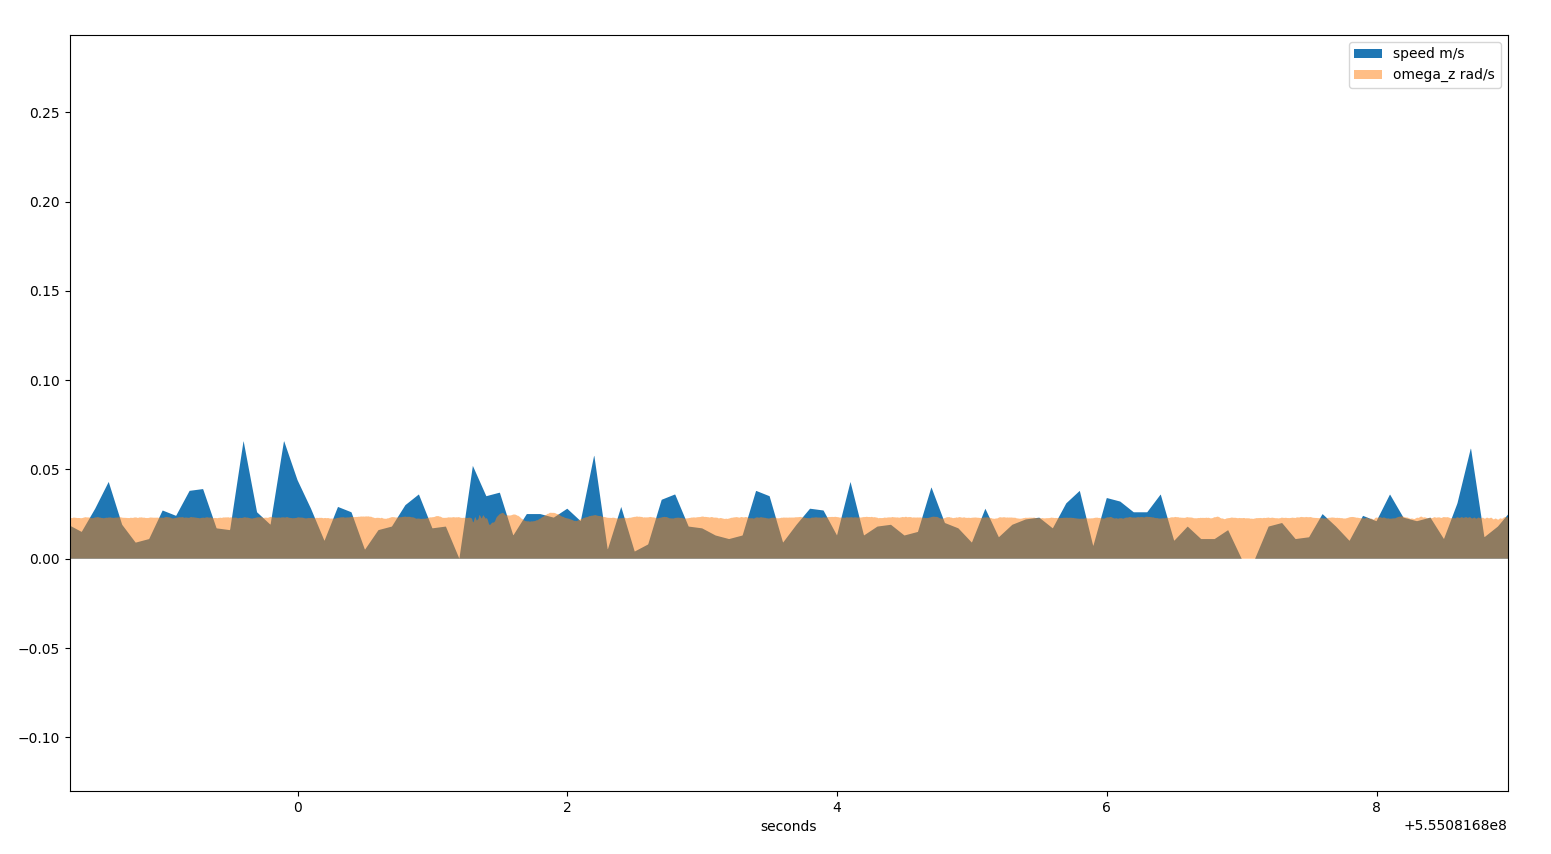
\includegraphics[width=\textwidth]{gyro_drift.png}
\caption{Data from stopped vehicle. Linear speed is near zero but gyroscope measure a non negligible angular speed}
\end{figure}

\section{Noise reduction}
Sensors are subject to noise, in data analyzed for this project I expecially found spikes without correlation to reality.
There are various technique to remove that, the one I used is the rolling average. \\
Given a series $s$ the \textit{centered} rolling average with a window size of $w$ is definied as:
$$ v_i = \frac{1}{w} \sum_{j=0}^{\frac{w}{2}}v_j \sum_{j=\frac{w}{2}}^{w}v_j $$
where $v_i$ is the element of series $s'$, that is $s$ with centered rolling average applied.
The choice of a value for window size is important. A too small value can lead to a too high noise left, while a too high windows size value can lead to \textit{flattening} and reduction of measured value. For example with a too high value an acceleration start to be measured before it actually exist and overall highest value is lower than in reality.

\section{Correction of vertical alignment}
Car's box vertical unalignment is corrected by looking at gravitational acceleration on stationary times. The used accelerometer doesn't remove it by default so I use it for ground truth of terrain position.
\begin{figure}[H]
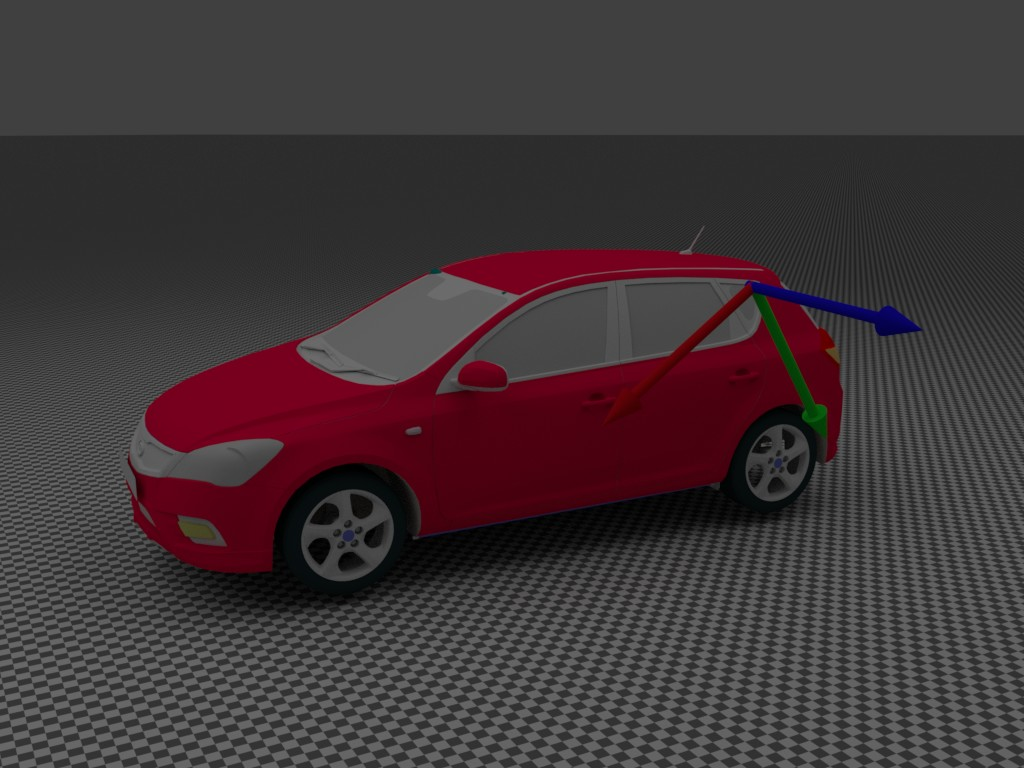
\includegraphics[width=\textwidth]{kia_bad_z_align.jpg}
\caption{Axes shows a sensor bad vertical alignment}
\end{figure}

Once obtained rotation angle, the program rotate both local acceleration and angular velocities. After having done that, if in a following stationary time a bad vertical alignment is still found, the program prints a warning on the console to notify that the box has misaligned during motion.

\section{Correction of horizontal alignment}
\begin{figure}[H]
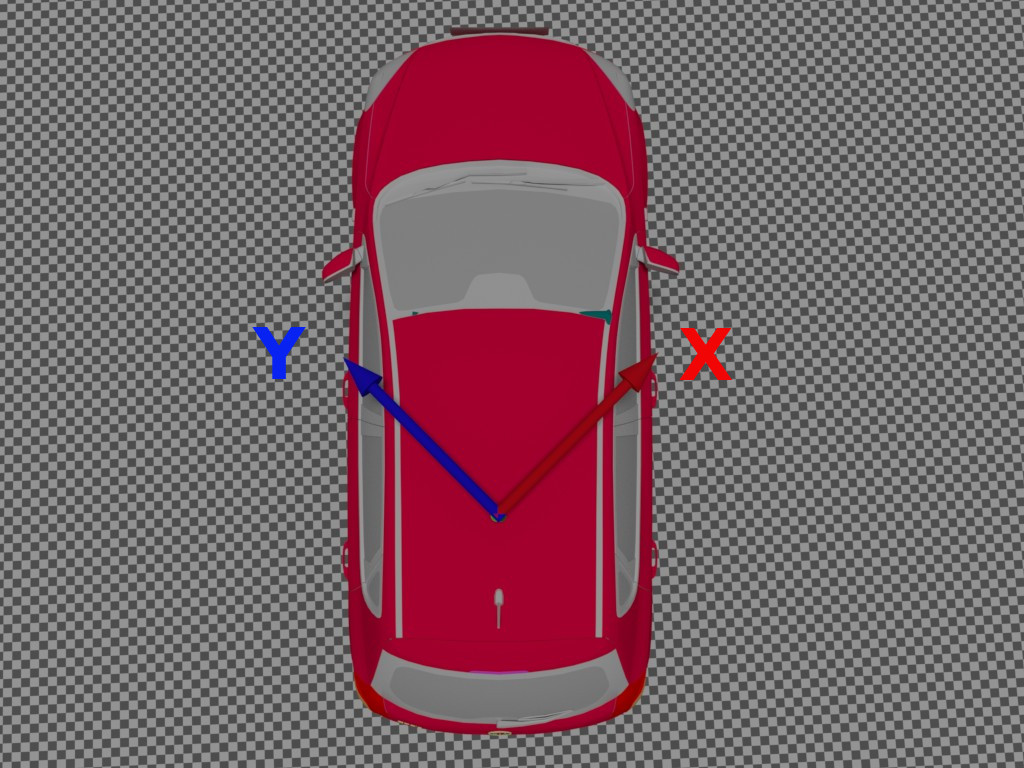
\includegraphics[width=\textwidth]{kia_bad_xy_align.jpg}
\end{figure}
Car's box horizontal unaligmnet is corrected by looking for situation where $a_x>0, \ a_y>0, \theta_z =0$. If this state exists, then or the car is sliding on ice or there is an unaligment on the $xy$ plane. Where, for example, an acceleration forward will be measured with both positive accelerations along x and y axis. 
Still in the situation described, the misaligment can be measured and corrected, still by rotating both local accelerations and angular velocities.

